\documentclass{article}
\usepackage{nips10submit_e,times}
%\documentstyle[nips07submit_09,times]{article}
\usepackage[square,numbers]{natbib}
\usepackage{amsmath, epsfig}
\usepackage{amsfonts}
\usepackage{subfigure}
\usepackage{graphicx}
\usepackage{amsfonts}
\usepackage{algorithm}
\usepackage{algorithmic}
\usepackage{easybmat}
\usepackage{footmisc}
\renewcommand\algorithmiccomment[1]{// \textit{#1}}
%
\newcommand{\ignore}[1]{}
\newcommand{\comment}[1]{}
\DeclareMathOperator*{\argmax}{arg\,max}

\title{Bayesian Nonparametric Ontology Learning}


\author{
Nicholas Bartlett \hspace{1cm} Matthew Hoffman \hspace{1cm} Frank Wood\\
Columbia University, New York, NY 10027, USA \\
\texttt{\{bartlett, xxx, fwood\}@stat.columbia.edu}
%\texttt{pfau@neurotheory.columbia.edu} 
%\texttt{\{bartlett,fwood\}@stat.columbia.edu} 
}

% The \author macro works with any number of authors. There are two commands
% used to separate the names and addresses of multiple authors: \And and \AND.
%
% Using \And between authors leaves it to \LaTeX{} to determine where to break
% the lines. Using \AND forces a linebreak at that point. So, if \LaTeX{}
% puts 3 of 4 authors names on the first line, and the last on the second
% line, try using \AND instead of \And before the third author name.

\newcommand{\fix}{\marginpar{FIX}}
\newcommand{\new}{\marginpar{NEW}}
\newcommand{\state}{q}
\newcommand{\symb}{\sigma}
\newcommand{\bmu}{\boldsymbol\mu}
\newcommand{\bphi}{\boldsymbol\phi}
\newcommand{\bpi}{\boldsymbol\pi}
\newcommand{\PY}{\textrm{PY}}
\newcommand{\geom}{\textrm{Geom}}
\newcommand{\unif}{\textrm{Unif}}
\newcommand{\perplexity}{\textrm{perp}}

\nipsfinalcopy

\begin{document}

\maketitle

% !TEX root = main.tex
\begin{abstract}
This shit rocks!
\end{abstract}
% !TEX root = main.tex
\section{Introduction}
\comment{All learning algorithms must strike a compromise between computational efficiency, model complexity, and generalization performance.  One extreme in terms of searching for minimally complex models is to search for the shortest computer program that can reproduce the observed data exactly. Unfortunately performing this search is well known to be computationally challenging, and, even if found, any single resulting program is not likely to generalize well given only a small number of observations\comment{generated by a complex mechanism}.   A mixture of such programs weighted by length, on the other hand, is the universal prior defined by Solomonoff \cite{Solomonoff1964,Solomonoff1978} and has good theoretical generalization properties.  Of course, given that searching for a single such program is costly, learning a mixture of programs becomes practically impossible.  

The focus of this paper is a similar in spirit but restricts the search in ways that render our approach computable.  Instead of learning a mixture of programs that can reproduce the data exactly, we, in effect, learn a mixture of probabilistic deterministic finite automata (PDFA), each of which can reproduce the data exactly.   We do this using a novel Bayesian framework for PDFA learning.  In this framework we first specify a prior over the parameters of a single large PDFA that encourages state reuse.  The inductive bias introduced by the prior can be interpreted as a kind of soft constraint that limits the number of states actually used by the PDFA to generate the observed data (its ``complexity'').   Being a Bayesian approach, we retain and average over our uncertainty about both the cardinality of states in the automata used to generate the data, the links between those states, and the emission distributions.  The posterior distribution over PDFA parameter settings can be interpreted as an infinite mixture over PDFAs.  A set of samples drawn from this distribution via, for instance, Markov chain Monte Carlo (MCMC) can be interpreted as a finite sample approximation to this infinite mixture, where again each sample is a PDFA of potentially varying complexity.  When performing inference we average over this posterior distribution, yielding a novel approach to smoothing over PDFAs, a technique known to produce good generalization results  \cite{pdfa_smoothing_approaches}.} % with a different number of states (only those that are used to generate the data matter), different emission distributions, and so forth.  
%The expressivity of a single PDFA with, to be redundant but necessarily pedantic, a finite number of states, is restrictive.  A mixture of PDFAs is less restrictive, in fact, it is know

The focus of this paper is a novel Bayesian framework for learning with probabilistic deterministic finite automata (PDFA) \cite{Rabin1963}.  A PDFA is a generative model for sequential data (PDFAs are reviewed in  Section \ref{sec:PDFA}).  Intuitively a PDFA is similar to a hidden Markov model (HMM) \cite{Rabiner1989} in that it consists of a set of states, each of which when visited emits a symbol according to an emission probability distribution.  It differs from an HMM in how state-to-state transitions occur; transitions are deterministic in a PDFA and nondeterministic in an HMM.  

In our framework for learning with PDFAs we specify a prior over the parameters of a single large PDFA that encourages state reuse.  The inductive bias introduced by the PDFA prior provides a soft constraint on the number of states used to generate the data.  We take the limit as the number of states becomes infinite, yielding a model we call the probabilistic deterministic infinite automata (PDIA).  

Given a finite training sequence, the PDIA posterior distribution is an infinite mixture of PDFAs.  Samples from this distribution form a finite sample approximation to this infinite mixture, and can be drawn via Markov chain Monte Carlo (MCMC) \cite{Gelman1995}.  Using such a mixture we can average over our uncertainty about the model parameters (including state cardinality) in a Bayesian way during prediction and other inference tasks.  We find that averaging over a finite number of PDFAs trained on naturalistic data leads to better predictive performance than using a single ``best'' PDFA.  

We chose to investigate learning with PDFAs because they are intermediate in expressive power between HMMs and finite-order Markov models, and thus strike a good balance between generalization performance and computational efficiency.  A single PDFA is known to have relatively limited expressivity.  We argue in \ref{sec:theory} that a finite mixture of PDFAs has greater expressivity than that of a single PDFA but is not as expressive as a probabilistic nondeterministic finite automata (PNFA)\footnote{PNFAs with no final probability are equivalent to hidden Markov models \cite{Dupont2005} \label{fn:pnfa}} .  A PDIA is clearly highly expressive; an infinite mixture over the same is even more so.  Even though ours is a Bayesian approach to PDIA learning, in practice we only ever deal with a finite approximation to the full posterior and thus limit our discussion to finite mixtures of PDFAs.

While model expressivity is a concern, computational considerations often dominate model choice.  We show that prediction in a trained mixture of PDFAs can have lower asymptotic cost than forward prediction in the PNFA/HMM\comment{\footref{fn:pnfa}} class of models.  We also present evidence that averaging over PDFAs gives predictive performance superior to HMMs trained with standard methods on naturalistic data.  We find that PDIA predictive performance is competitive with that of fixed-order, smoothed Markov models with the same number of states.  While sequence learning approaches such as the HMM and smoothed Markov models are well known and now highly optimized, our PDIA approach to learning is novel and is amenable to future improvement.  

Section \ref{sec:PDFA} reviews PDFAs, Section \ref{sec:BPDFAs} introduces Bayesian PDFA inference, Section \ref{sec:results} presents experimental results on DNA and natural language, and Section \ref{sec:theory} discusses related work on PDFA induction and the theoretical expressive power of mixtures of PDFAs.
In Section \ref{sec:discussion} we discuss ways in which PDIA predictive performance might be improved in future research.

\comment{
 We wish to learn a mixture of probabilistic deterministic finite automata any of which could have generated the observed data.  of Bayesian learning of a probabilistic deterministic infinite automata (PDIA).  A probabilistic deterministic automata with an infinite number of states is a  a class of models that includes variable and fixed order Markov models as a special case, as well as simpler models.  

%At a high level, a PDFA can be thought of as a hidden Markov model for which, given an observed sequence, there is only one possible path through the hidden states.  A more formal definition follows in section 2.
We motivate our choice of model class several ways.  First, it can be shown by a simple argument that, given an infinite and stationary sequence, the minimal sufficient statistics of the past for predicting the future form a PDFA \cite{Crutchfield1999}.  That is, given two pasts that map to the same statistic, the concatenation of those pasts with the same symbol will map to the same statistic.  This is not the case in general hidden Markov models, where many transitions are possible from a hidden state, though observed data may change the posterior probability of those transitions.  Existing algorithms for learning these statistics use tests that have asymptotic guarantees but may not work well for reasonable amounts of data \cite{Shalizi2004}.

Another argument is that we are trying to generalize the class of variable-length Markov models, which have had great empirical success in sequence prediction.

N-gram models have had great empirical success in sequence prediction.  However, there is no clear way to trade off model complexity with prediction accuracy.  In extensions to n-gram models which can learn from arbitrarily long contexts, the model complexity will grow without bound, even for trivially simple sequences such as repetitions of a few characters.  Bounded memory models perform well in practice, but we would much prefer to learn a model that is as small as possible for very simple data, while growing large for more complex data.  A natural class of models to explore is probabalistic deterministic finite automata (PDFA), which contains n-grams as a special case, as well as simpler models.  We define a prior over PDFAs with a finite number of states and describe a Metropolis-Hastings algorithm to generate samples from the posterior.  We then generalize to the case of PDFAs with a (potentially) infinite number of states and show that the generative model is a type of Hierarchical Dirichlet Process (HDP).  We then (I hope!) describe a state splitting/merging algorithm for posterior inference that mixes more efficiently than the original Metropolis-Hastings algorithm, and show that it defines a natural hierarchy of states for smoothing (fingers crossed...)  The set of strings produced by a PDFA constitutes a probabilistic regular language, thus our inference procedure can also be viewed as a non-greedy algorithm for regular grammar induction.

Finally, }

\section{Model Definition}

\begin{figure}[htbp]
\centering
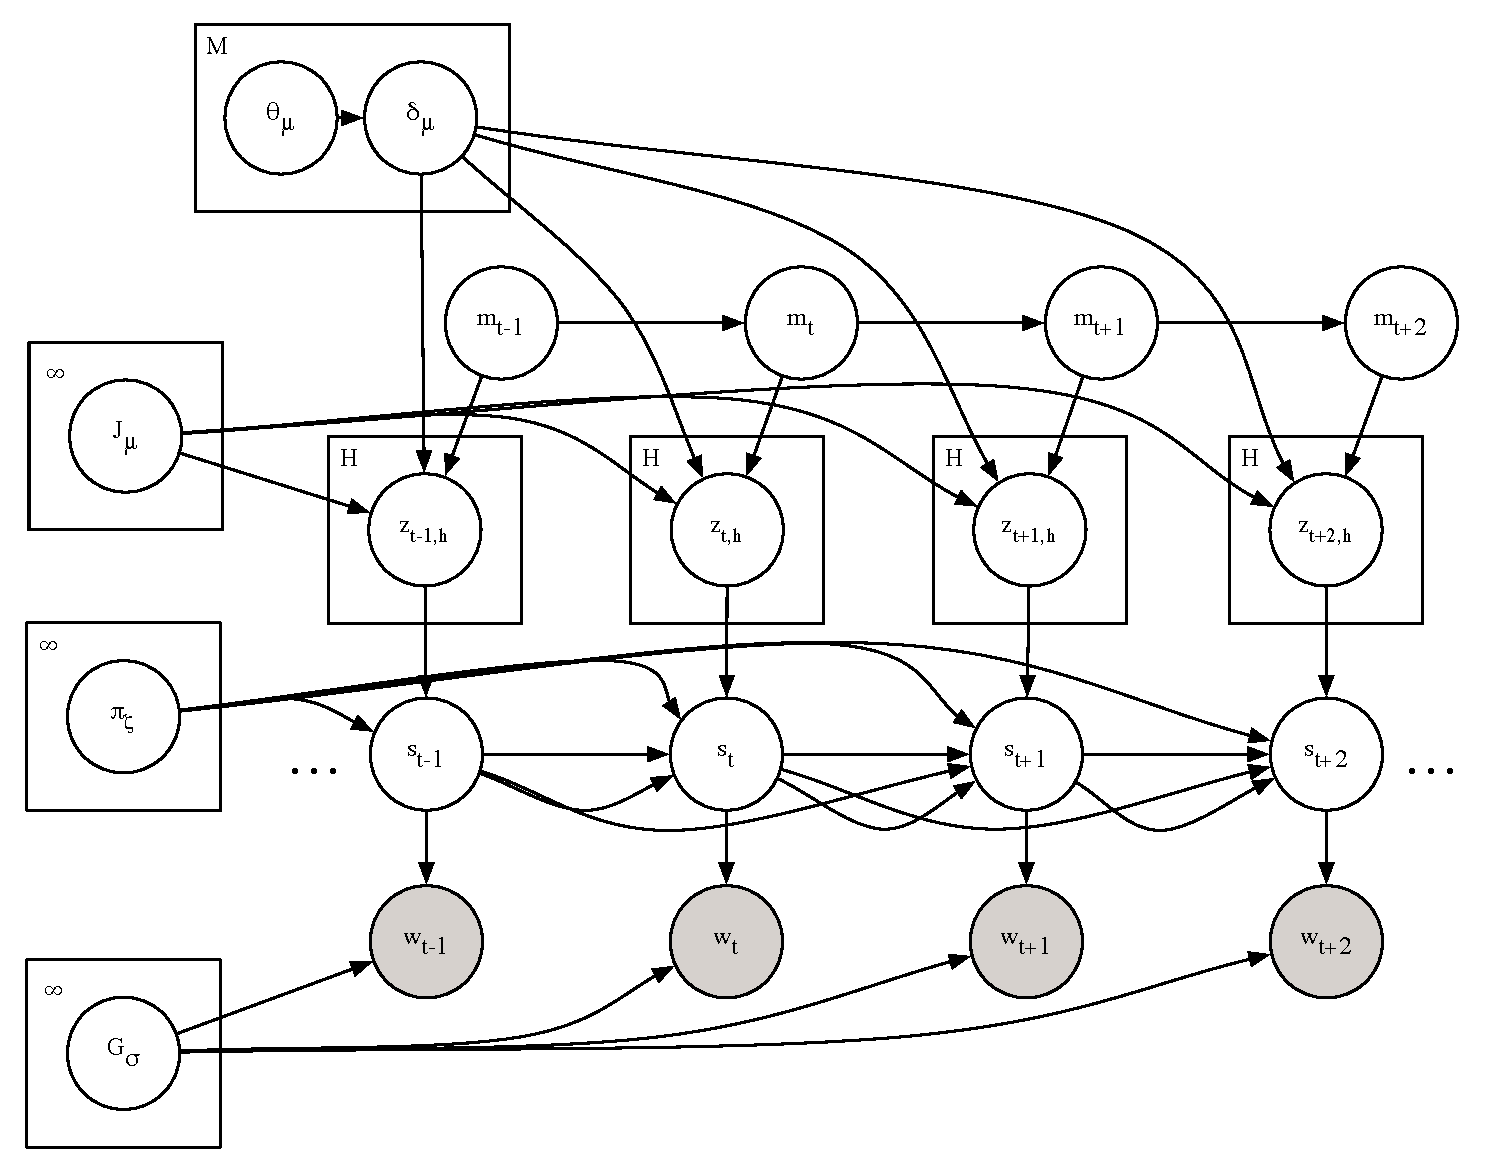
\includegraphics[width=1\textwidth]{figures/graphicalmodel}
\caption{Graphical model. \label{fig:graphicalmodel}}
\end{figure}

%% For each word $x_t$, we assume that there is a corresponding binary
%% vector $s_t \in \mathcal{S} \equiv \{0, 1\}^*$.

%% We assume that at each time $t$, a binary vector $z_t$ is drawn
%% according to a process that will be defined below. Conditioned on this
%% vector $z_t$, a corresponding word $w_t$ is drawn according to a
%% hierarchical Pitman-Yor process

At each time step $t$, a Deterministic Infinite Automaton (DIA) $m_t
\in \mathcal{M}$ is chosen according to a Markov process:
\begin{equation}
J_\mu \sim \PY(1, 1, \unif(\mathcal{M}));\quad
m_t \sim J_{m_{t-1}}.
\end{equation}

For each Deterministic Infinite Automaton (DIA) $\mu \in \mathcal{M}
\equiv \{1,\ldots,M\}$, we assume that the parameters $\delta_\mu$
associated with that that DIA are sampled according to the following
process:
\begin{equation}
\theta_{\mu,\epsilon} \sim \PY(c^{\delta}, d^{\delta}_{0},\geom(q)); \quad
\theta_{\mu,\sigma} \sim \PY(c^{\delta}, d^{\delta}_{|\sigma|},
\theta_{\mu,\gamma(\sigma)}); \quad
\delta_{\mu,\zeta,\sigma} \sim \theta_{\mu,\sigma}.
\end{equation}
$\gamma(\sigma)$ is an operator that removes the least significant bit
in the binary vector $\sigma$; for example, $\gamma(011001)=01100$.

Given a sequence of the $H$ binary vectors $s_{t-H:t-1}$ preceding
time $t$, the DIA $m_t$ generates a sequence of states $z_{t,-H:0}$
according to the following deterministic program:
\begin{equation}
z_{t,-H} = 0; \quad
\textrm{for } h \in \{-H+1,\ldots,0\}, z_{t,h} = \delta_{m_t, z_{t,h-1}, s_{t+h}}.
\end{equation}
Shared across all of these DIA is a set of (a countably infinite
number of) emission distributions $\pi_{\zeta}$ over binary
vectors. Each $\pi_{\zeta}$ is defined by a set of $r, l,$ and $s$
variables drawn from a Pitman-Yor process:
\begin{equation}
\begin{split}
\{r_{0,\sigma}, l_{0,\sigma}, u_{0,\sigma}\} &\sim \PY(c_0^\pi, d^\pi_{0}, 
\{\frac{1-\beta}{2}, \frac{1-\beta}{2}, \beta\}); \\
\{r_{\zeta,\sigma}, l_{\zeta,\sigma}, u_{\zeta,\sigma}\} &\sim 
\PY(c_1^\pi, d^\pi_{1}, \{r_{0,\sigma}, l_{0,\sigma}, u_{0,\sigma}\}).
\end{split}
\end{equation}
Given $r, l,$ and $s$, each of these distributions generates binary
state vectors $\sigma$ according to the following process:
\begin{enumerate}
\item Initialize $\sigma$ to the empty vector $\epsilon$.
\item Until the process is stopped:
  \begin{enumerate}
  \item Either append a 1 to $\sigma$ (with probability $r_{z_{t,0}, \sigma}$),
    append a 0 to $\sigma$ (with probability $l_{z_{t,0}, \sigma}$), or
    stop the process (with probability $u_{z_{t,0},\sigma}$).
  \end{enumerate}
\end{enumerate}
%% \begin{equation}
%% \begin{split}
%% s_{t,0} &\sim \{r_{z_{t,0}, \epsilon}, l_{z_{t,0}, \epsilon}, 
%% s_{z_{t,0}, \epsilon}\}; \\
%% s_{t,b} &\sim \{r_{z_{t,0}, s_{t,1:b-1}}, l_{z_{t,0}, s_{t,1:b-1}}, 
%% s_{z_{t,0}, s_{t,1:b-1}}\}
%% \end{split}
%% \end{equation}
We denote the probability of generating a particular binary vector
$\sigma$ under the emission distribution indexed by $\zeta$ as
$\pi_{\zeta}(\sigma)$. Thus, we can write
\begin{equation}
s_t \sim \pi_{z_{t,0}}.
\end{equation}
Conditioned on the latent binary state vector $s_t$ for time $t$, we
draw word $w_t$ according to a hierarchical Pitman-Yor process:
\begin{equation}
\begin{split}
G_{\epsilon} \sim \PY(c^G, d^G_{0},\unif(1,\ldots,W)); \quad
G_\sigma \sim \PY(c^G, d^G_{|\sigma|},G_{\gamma(\sigma)}); \quad
w_t \sim G_{s_t}.
\end{split}
\end{equation}
$W$ is the size of the vocabulary.


\section{Experiments}

We ran several experiments to evaluate BNOL's usefulness for analyzing
text documents. In the first experiment, we tested BNOL's ability to
recover structure from a synthetic dataset. In the second experiment,
we evaluated the quality of the ontologies discovered by
BNOL. Finally, we evaluated BNOL's ability to accurately predict the
next entry in a stream of text.

\subsection{Synthetic Data}
We created a simple artificial ontology (displayed in figure
\ref{fig:fakeontology}) and generated some text using it. [Insert
  actual fake generative process here.] We then ran the MCMC algorithm
described in section \ref{sec:inference} on the synthetic document.
The ontology discovered by BNOL is shown in figure
\ref{fig:bnolsynth}. The algorithm has done a good job of recovering
the ontological structure in the synthetic dataset.

\subsection{Evaluating Ontologies}
To evaluate the quality of the ontologies discovered by BNOL on real
datasets, we analyzed the XXX corpus using the inference algorithm in
section \ref{sec:inference}. The ontology found by the model is shown
in figure \ref{fig:realontology}. [Discussion of the qualitative
  desiderata exhibited by the ontology, i.e., ``this totally worked.'']

[Quantitative evaluation of the ontology that showcases whatever BNOL
is actually good at, e.g. finding POS, etc.]

\subsection{Prediction}
In addition to being able to extract meaningful structure from text
data, BNOL defines a predictive model of streaming text that can be
used to do language modeling (e.g. to facilitate speech recognition
\cite{???}) or data compression \cite{???}.

We evaluated BNOL's ability to predict the next word in a sequence
based on the previous words. Our measure of predictive performance
is perplexity, which is defined as
\begin{equation}
\perplexity(x, x_\textrm{train}) \equiv
\exp\left\{-\frac{1}{N}\sum_{i=1}^N\log p(x_i|x_{1:i-1},
x_\textrm{train})\right\}.
\end{equation}

[How well we do. Compare to infinite sequence memoizer?]

%% % !TEX root = main.tex
\begin{abstract}
This shit rocks!
\end{abstract}

%% % !TEX root = main.tex
\section{Introduction}
\comment{All learning algorithms must strike a compromise between computational efficiency, model complexity, and generalization performance.  One extreme in terms of searching for minimally complex models is to search for the shortest computer program that can reproduce the observed data exactly. Unfortunately performing this search is well known to be computationally challenging, and, even if found, any single resulting program is not likely to generalize well given only a small number of observations\comment{generated by a complex mechanism}.   A mixture of such programs weighted by length, on the other hand, is the universal prior defined by Solomonoff \cite{Solomonoff1964,Solomonoff1978} and has good theoretical generalization properties.  Of course, given that searching for a single such program is costly, learning a mixture of programs becomes practically impossible.  

The focus of this paper is a similar in spirit but restricts the search in ways that render our approach computable.  Instead of learning a mixture of programs that can reproduce the data exactly, we, in effect, learn a mixture of probabilistic deterministic finite automata (PDFA), each of which can reproduce the data exactly.   We do this using a novel Bayesian framework for PDFA learning.  In this framework we first specify a prior over the parameters of a single large PDFA that encourages state reuse.  The inductive bias introduced by the prior can be interpreted as a kind of soft constraint that limits the number of states actually used by the PDFA to generate the observed data (its ``complexity'').   Being a Bayesian approach, we retain and average over our uncertainty about both the cardinality of states in the automata used to generate the data, the links between those states, and the emission distributions.  The posterior distribution over PDFA parameter settings can be interpreted as an infinite mixture over PDFAs.  A set of samples drawn from this distribution via, for instance, Markov chain Monte Carlo (MCMC) can be interpreted as a finite sample approximation to this infinite mixture, where again each sample is a PDFA of potentially varying complexity.  When performing inference we average over this posterior distribution, yielding a novel approach to smoothing over PDFAs, a technique known to produce good generalization results  \cite{pdfa_smoothing_approaches}.} % with a different number of states (only those that are used to generate the data matter), different emission distributions, and so forth.  
%The expressivity of a single PDFA with, to be redundant but necessarily pedantic, a finite number of states, is restrictive.  A mixture of PDFAs is less restrictive, in fact, it is know

The focus of this paper is a novel Bayesian framework for learning with probabilistic deterministic finite automata (PDFA) \cite{Rabin1963}.  A PDFA is a generative model for sequential data (PDFAs are reviewed in  Section \ref{sec:PDFA}).  Intuitively a PDFA is similar to a hidden Markov model (HMM) \cite{Rabiner1989} in that it consists of a set of states, each of which when visited emits a symbol according to an emission probability distribution.  It differs from an HMM in how state-to-state transitions occur; transitions are deterministic in a PDFA and nondeterministic in an HMM.  

In our framework for learning with PDFAs we specify a prior over the parameters of a single large PDFA that encourages state reuse.  The inductive bias introduced by the PDFA prior provides a soft constraint on the number of states used to generate the data.  We take the limit as the number of states becomes infinite, yielding a model we call the probabilistic deterministic infinite automata (PDIA).  

Given a finite training sequence, the PDIA posterior distribution is an infinite mixture of PDFAs.  Samples from this distribution form a finite sample approximation to this infinite mixture, and can be drawn via Markov chain Monte Carlo (MCMC) \cite{Gelman1995}.  Using such a mixture we can average over our uncertainty about the model parameters (including state cardinality) in a Bayesian way during prediction and other inference tasks.  We find that averaging over a finite number of PDFAs trained on naturalistic data leads to better predictive performance than using a single ``best'' PDFA.  

We chose to investigate learning with PDFAs because they are intermediate in expressive power between HMMs and finite-order Markov models, and thus strike a good balance between generalization performance and computational efficiency.  A single PDFA is known to have relatively limited expressivity.  We argue in \ref{sec:theory} that a finite mixture of PDFAs has greater expressivity than that of a single PDFA but is not as expressive as a probabilistic nondeterministic finite automata (PNFA)\footnote{PNFAs with no final probability are equivalent to hidden Markov models \cite{Dupont2005} \label{fn:pnfa}} .  A PDIA is clearly highly expressive; an infinite mixture over the same is even more so.  Even though ours is a Bayesian approach to PDIA learning, in practice we only ever deal with a finite approximation to the full posterior and thus limit our discussion to finite mixtures of PDFAs.

While model expressivity is a concern, computational considerations often dominate model choice.  We show that prediction in a trained mixture of PDFAs can have lower asymptotic cost than forward prediction in the PNFA/HMM\comment{\footref{fn:pnfa}} class of models.  We also present evidence that averaging over PDFAs gives predictive performance superior to HMMs trained with standard methods on naturalistic data.  We find that PDIA predictive performance is competitive with that of fixed-order, smoothed Markov models with the same number of states.  While sequence learning approaches such as the HMM and smoothed Markov models are well known and now highly optimized, our PDIA approach to learning is novel and is amenable to future improvement.  

Section \ref{sec:PDFA} reviews PDFAs, Section \ref{sec:BPDFAs} introduces Bayesian PDFA inference, Section \ref{sec:results} presents experimental results on DNA and natural language, and Section \ref{sec:theory} discusses related work on PDFA induction and the theoretical expressive power of mixtures of PDFAs.
In Section \ref{sec:discussion} we discuss ways in which PDIA predictive performance might be improved in future research.

\comment{
 We wish to learn a mixture of probabilistic deterministic finite automata any of which could have generated the observed data.  of Bayesian learning of a probabilistic deterministic infinite automata (PDIA).  A probabilistic deterministic automata with an infinite number of states is a  a class of models that includes variable and fixed order Markov models as a special case, as well as simpler models.  

%At a high level, a PDFA can be thought of as a hidden Markov model for which, given an observed sequence, there is only one possible path through the hidden states.  A more formal definition follows in section 2.
We motivate our choice of model class several ways.  First, it can be shown by a simple argument that, given an infinite and stationary sequence, the minimal sufficient statistics of the past for predicting the future form a PDFA \cite{Crutchfield1999}.  That is, given two pasts that map to the same statistic, the concatenation of those pasts with the same symbol will map to the same statistic.  This is not the case in general hidden Markov models, where many transitions are possible from a hidden state, though observed data may change the posterior probability of those transitions.  Existing algorithms for learning these statistics use tests that have asymptotic guarantees but may not work well for reasonable amounts of data \cite{Shalizi2004}.

Another argument is that we are trying to generalize the class of variable-length Markov models, which have had great empirical success in sequence prediction.

N-gram models have had great empirical success in sequence prediction.  However, there is no clear way to trade off model complexity with prediction accuracy.  In extensions to n-gram models which can learn from arbitrarily long contexts, the model complexity will grow without bound, even for trivially simple sequences such as repetitions of a few characters.  Bounded memory models perform well in practice, but we would much prefer to learn a model that is as small as possible for very simple data, while growing large for more complex data.  A natural class of models to explore is probabalistic deterministic finite automata (PDFA), which contains n-grams as a special case, as well as simpler models.  We define a prior over PDFAs with a finite number of states and describe a Metropolis-Hastings algorithm to generate samples from the posterior.  We then generalize to the case of PDFAs with a (potentially) infinite number of states and show that the generative model is a type of Hierarchical Dirichlet Process (HDP).  We then (I hope!) describe a state splitting/merging algorithm for posterior inference that mixes more efficiently than the original Metropolis-Hastings algorithm, and show that it defines a natural hierarchy of states for smoothing (fingers crossed...)  The set of strings produced by a PDFA constitutes a probabilistic regular language, thus our inference procedure can also be viewed as a non-greedy algorithm for regular grammar induction.

Finally, }
%% % !TEX root = main.tex
\section{Probabilistic Deterministic Finite Automata}
\label{sec:PDFA}

A PDFA is formally defined as a 5-tuple $M = (Q,\Sigma,\delta,\pi,\state_0)$, where $Q$ is a finite set of states, $\Sigma$ is a finite alphabet of observable symbols, $\delta\,:\,Q\times\Sigma\rightarrow Q$ is the transition function from a state/symbol pair to the next state, $\pi\,:\,Q\times\Sigma\rightarrow[0,1]$ is the probability of the next symbol given a state and $\state_0$ is the initial state.\footnote{In general $\state_0$ may be replaced by a distribution over initial states.  \comment{We are interested in inference when the path is known exactly, and so restrict ourselves to the case of a single initial state.}}  Throughout this paper we will use $i$ to index elements of $Q$, $j$ to index elements of $\Sigma$, and $t$ to index elements of an observed string.  For example, $\delta_{ij}$ is shorthand for $\delta(\state_i,\symb_j)$, where $\state_i \in Q$ and $\symb_j \in \Sigma$.

Given a state $\state_i$, the probability that the next symbol takes the value $\symb_j$ is given by $\pi(\state_i,\symb_j)$.  We use the shorthand $\bpi_{q_i}$ for the state-specific discrete distribution over symbols for state $\state_i$.  We can also write $\sigma|\state_i \sim \bpi_{q_i}$ where $\sigma$ is a random variable that takes values in $\Sigma$.  Given a state $\state_i$ and a symbol $\symb_j$, however, the next state $\state_{i'}$ is {\it deterministic}: $\state_{i'} = \delta(\state_i,\symb_j).$   Generating from a PDFA involves first generating a symbol stochastically given the state the process is in: $x_t|\q_t \sim \bpi_{\q_t}$ where $\q_t \in Q$ is the state at time $t$.  Next, given $\q_t$ and $x_t$ transitioning deterministically to the next state: $\q_{t+1} = \delta(\q_t,x_t)$.  This is the reason for the confusing ``probabilistic deterministic'' name for these models.  Turning this around, given data, $q_0$, and $\delta$, there is no uncertainty about the path through the states.  This is a primary source of computational savings relative to HMMs.

PDFAs are more general than $n$th-order Markov models (i.e. $m$-gram models, $m=n+1$), but less expressive than hidden Markov models (HMMs)\cite{Dupont2005}.  For the case of $n$th-order Markov models, we can construct a PDFA with one state per suffix $x_1 x_2 \ldots x_n$.  Given a state and a symbol $x_{n+1}$, the unique next state is the one corresponding to the suffix $x_2 \ldots x_{n+1}$.  Thus $n$th-order Markov models are a subclass of PDFAs with $\mathcal{O}(|\Sigma|^n)$ states.  For an HMM, given data and an initial distribution over states, there is a posterior probability for every path through the state space.  PDFAs are those HMMs for which, given a unique start state, the posterior probability over paths is degenerate at a single path.  As we explain in Section \ref{sec:theory}, mixtures of PDFAs are strictly more expressive than single PDFAs, but still less expressive than PNFAs.

%% % !TEX root = main.tex
\section{Bayesian PDFA Inference}
\label{sec:BPDFAs}

We start our description of Bayesian PDFA inference by defining a prior distribution over the parameters of a finite PDFA.  We then show how to analytically marginalize nuisance parameters out of the model and derive a Metropolis-Hastings sampler for posterior inference using the resulting collapsed representation.  We discuss the limit of our model as the number of states in the PDFA goes to infinity.  We call this limit the probabilistic deterministic infinite automaton (PDIA).  We develop a PDIA sampler that carries over from the finite case in a natural way.

%, and show that many of the elements of the transition matrix can be ignored without affecting the correctness of sampling

\subsection{A PDFA Prior}

We assume that the set of states $Q$, set of symbols $\Sigma$, and initial state $q_0$ of a PDFA are known but that the transition and emission functions are unknown.  The PDFA prior then consists of a prior over both the transition function $\delta$ and the emission probability function $\pi$.  In the finite case $\delta$ and $\pi$ are representable as finite matrices, with one column per element of $\Sigma$ and one row per element of $Q$.  For each column $j$ ($j$ co-indexes columns and set elements) of the transition matrix $\delta$, our prior stipulates that the elements of that column are  i.i.d. draws from a discrete distribution $\bphi_j$ over $Q$, that is, $\delta_{ij} \sim [\bphi_1,\ldots,\bphi_{|\Sigma|}], \; 0 \leq i\leq|Q|-1$.  The $\bphi_j$ represent transition tendencies given a symbol, if the $i$th element of $\bphi_{j}$ is large then state $q_i$ is likely to be transitioned to anytime the last symbol was $\symb_j$.   The $\bphi_{j}$'s are themselves given a shared Dirichlet prior with parameters $\alpha\bmu$, where $\alpha$ is a concentration and $\bmu$ is a template transition probability vector.   If the $i$th element of $\bmu$ is large then the $i$th state is likely to be transitioned to regardless of the emitted symbol.  We place a uniform Dirichlet prior on $\bmu$ itself, with $\gamma$ total mass and average over $\bmu$ during inference.  This hierarchical Dirichlet construction encourages both general and context specific state reuse.
 We also place a uniform Dirichlet prior over the per-state emission probabilities $\bpi_{q_i}$ with $\beta$ total mass which smooths emission distribution estimates.  Formally:
%
\begin{eqnarray}
\bmu|\gamma,|Q| & \sim & \mathrm{Dir}\left(\gamma/|Q|,\ldots,\gamma/|Q|\right) \label{gen:mu}  \\
\bphi_{j}|\alpha,\bmu  & \sim & \mathrm{Dir}(\alpha\bmu) \label{gen:phi} \\
\bpi_{q_i}|\beta,|\Sigma| & \sim & \mathrm{Dir}(\beta/|\Sigma|,\ldots,\beta/|\Sigma|) \label{gen:pi} \nonumber \\
\delta_{ij} & \sim & \bphi_{j} \label{gen:delta} \nonumber
\end{eqnarray}
%
where $0 \leq i \leq |Q|-1$ and $1 \leq j \leq |\Sigma|$.  Given a sample from this model we can run the PDFA to generate a sequence of $T$ symbols.  Using $\q_t$ to denote the state of the PDFA at position $t$ in the sequence:
%
\begin{equation}
\q_0 = \state_0, \qquad
x_0 \sim \bpi_{q_0}, \qquad
\q_t = \delta(\q_{t-1},x_{t-1}), \qquad
x_t \sim \bpi_{\q_t} \label{gen} \nonumber
\end{equation}
%
We choose this particular inductive bias, with transitions tied together within a column of $\delta$, because we wanted the most recent symbol emission to be informative about what the next state is.  If we instead had a single Dirichlet prior over all elements of $\delta$, transitions to a few states would be highly likely no matter the context and those states would dominate the behavior of the automata.  If we tied together rows of $\delta$ instead of columns, being in a particular state would tell us more about the sequence of states we came from than the symbols that got us there.  
%As we would like states to be good statistics of the past for predicting the future, a bias that depends on the most recent symbol is preferable.

 Note that this prior stipulates a fully connected PDFA in which all states may transition to all others and all symbols may be emitted from each state.  This is slightly different that the canonical finite state machine literature where sparse connectivity is usually the norm.

\subsection{PDFA Inference}

Given observational data, we are interested in learning a posterior distribution over PDFAs.  We do this by GIbbs sampling the transition matrix $\delta$ with $\bpi$ and $\bphi_j$ integrated out.  To start inference we need the likelihood function for a fixed PDFA; it is given by
%
\[ p(x_{0:T}|\pi,\delta) = \pi(\q_0,x_0)\prod_{t=1}^T \pi(\q_t,x_t) \label{x:def}. \]
%
Remember that $\q_t | \q_{t-1}, x_{t-1}$ is deterministic given the transition function $\delta$. 
We can marginalize $\pi$ out of this expression and express the likelihood of the data in a form that depends only on the counts of symbols emitted from each state.  Define the count matrix $c$ for the sequence $x_{0:T}$ and transition matrix $\delta$ as $c_{ij} = \sum_{t=0}^T I_{ij}(\q_t,x_t)$, where $I_{ij}(\q_t,x_t)$ is an indicator function for the automaton being in state $q_i$ when it generates $x_t$, i.e. $\q_t = q_i$ and $x_t = \sigma_j$. This matrix $c = [c_{ij}]$ gives the number of times each symbol is emitted from each state.  Due to multinomial-Dirichlet conjugacy we can express the probability of a sequence given the transition function $\delta$, the count matrix $c$ and $\beta$:
%
\begin{eqnarray}
 p(x_{0:T}|\delta,c,\beta) & = & \int p(x_{0:T}|\pi,\delta) p(\pi|\beta) d\pi \label{x:factor} %\nonumber \\
 %& = &  \prod_{i=0}^{|Q|-1} \frac{\Gamma(\beta)}{\Gamma(\frac{\beta}{|\Sigma|})^{|\Sigma|}} \int\pi_{i1}^{\frac{\beta}{|\Sigma|}+c_{i1}-1} \pi_{i2}^{\frac{\beta}{|\Sigma|}+c_{i2}-1} \ldots \pi_{i|\Sigma|}^{\frac{\beta}{|\Sigma|}+c_{i|\Sigma|}-1} d\bpi_i \label{x:int}\\
= \prod_{i=0}^{|Q|-1} \frac{\Gamma(\beta)}{\Gamma(\frac{\beta}{|\Sigma|})^{|\Sigma|}} \frac{\prod_{j=1}^{|\Sigma|}\Gamma(\frac{\beta}{|\Sigma|} + c_{ij})}{\Gamma(\beta + \sum_{j=1}^{|\Sigma|} c_{ij})} \label{x:end}
 \end{eqnarray}
 %
If the transition matrix $\delta$ is observed we have a closed-form expression for its likelihood given $\bmu$ with all $\bphi_j$'s marginalized out.  Let $v_{ij}$ be the number of times state $q_i$ is transitioned to given that $\sigma_j$ was the last symbol emitted, i.e.~$v_{ij}$ is the number of times $\delta_{i'j} = q_i$ for all states $i'$ in the column $j$. %, that is, $v_{ij} = \displaystyle\sum_{i' = 0}^{|Q|-1} I_{i}(\delta_{i'j})$, $I_i(q_{i'})$ being the indicator function that is only 1 when $q_i' = q_i$. 
%Given $\bmu$, we can integrate out $\phi$ and express t
The marginal likelihood of $\delta$ in terms of $\bmu$ is then:
 %
 \begin{eqnarray}
 p(\delta|\bmu,\alpha) & = & \int p(\delta|\phi)p(\phi|\bmu,\alpha) d\phi %\label{delta:factor}
%  & = & \prod_{j=1}^{|\Sigma|} \frac{\Gamma(\alpha)}{\prod_{i=0}^{|Q|-1}\Gamma(\alpha\mu_i)} \int \phi_{0j}^{\alpha\mu_0+v_{0j}-1} \phi_{1j}^{\alpha\mu_1+v_{1j}-1} \ldots \phi_{|Q|-1,j}^{\alpha\mu_{|Q|-1}+v_{|Q|-1,j}-1} d\bphi_j \label{delta:int}\\
   =   \prod_{j=1}^{|\Sigma|} \frac{\Gamma(\alpha)}{\prod_{i=0}^{|Q|-1}\Gamma(\alpha\mu_i)} \frac{\prod_{i=0}^{|Q|-1} \Gamma(\alpha\mu_i + v_{ij})}{\Gamma(\alpha + |Q|)} \label{delta:end}
  \end{eqnarray}
%
%\begin{eqnarray}
%p(\bmu|\delta,\alpha, \gamma) & = & \frac{p(\delta|\bmu,\alpha)p(\bmu|\gamma)}{\int p(\delta|\bmu,\alpha)p(\bmu|\gamma) d\bmu}
%\end{eqnarray}
% 
We perform posterior inference in the finite model by sampling elements of $\delta$ and the vector $\bmu$.  %From the formulas above, it is straightforward to write down the conditional probability for one element of the transition matrix $\delta$. 
One can sample $\delta_{ij}$ given the rest of the matrix $\delta_{-ij}$ using 
%
\begin{equation}
p(\delta_{ij}|\delta_{-ij},x_{0:T},\bmu,\alpha) \propto p(x_{0:T}|\delta_{ij},\delta_{-ij})p(\delta_{ij}|\delta_{-ij},\bmu,\alpha) \label{delta:cond}
\end{equation}
%
Both terms on the right hand side of this equation have closed-form expressions, the first given in \eqref{x:end}.  The second can be found from \eqref{delta:end} and is
%
\begin{equation}
P(\delta_{ij} = q_{i'}|\delta_{-ij},\alpha,\bmu) = \frac{\alpha\mu_{i'} + v_{i'j}}{\alpha + |Q| - 1} \label{delta:pred}
\end{equation}
%
where $v_{i'j}$ is the number of elements in column $j$ equal to $q_{i'}$  excluding $\delta_{ij}$.  As $|Q|$ is finite, we compute \eqref{delta:cond} for all values of $\delta_{ij}$ and normalize to produce the required conditional probability distribution.

Note that in \eqref{x:end}, the count matrix $c$ may be profoundly impacted by changing even a single element of $\delta$.  The values in $c$ depend on the specific sequence of states the automata used to generate $x$.  Changing the value of a single element of $\delta$ affects the state trajectory the PDFA must follow to generate $x_{0:T}$.  %By changing $\delta_{ij}$, the set of states visited and the order in which those states are visited after the first time $q_i$ emits $\sigma_j$ are affected. 
 Among other things this means that some elements of $c$ that were nonzero may become zero, and vice versa.

We can reduce the computational cost of inference by deleting transitions $\delta_{ij}$ for which the corresponding counts $c_{ij}$ become 0.  In practical sampler implementations this means that one need not even represent transitions corresponding to zero counts.  The likelihood of the data \eqref{x:end} does not depend on the value of $\delta_{ij}$ if symbol $\sigma_j$ is never emitted while the machine is in state $\state_i$.   In this case sampling from \eqref{delta:cond} is the same as sampling without conditioning on the data at all.  Thus, if while sampling we change some transition that renders $c_{ij}=0$ for some values for each of $i$ and $j$, we can delete $\delta_{ij}$ until another transition is changed such that $c_{ij}$ becomes nonzero again, when we sample $\delta_{ij}$ anew.  Under the marginal joint distribution of a column of $\delta$ the row entries in that column are exchangeable, and so deleting an entry of $\delta$ has the same effect as marginalizing it out.  When all $\delta_{ij}$ for some state $q_i$ are marginalized out, we can say the state itself is marginalized out.
%The conditional distribution of the other elements of $\delta_{i'j}, \; i'\neq i, 0\leq i'\leq|Q|-1$ conditioned on the model where superfluous transitions are marginalized out.  
When we delete an element from a column of $\delta$, we replace the $|Q| - 1$ in the denominator of \eqref{delta:pred} with $D^+_j = \sum_{i=0}^{|Q|-1}I(v_{ij}\neq0)$, the number of entries in the $j$th column of $\delta$ that are {\em not} marginalized out yielding
\begin{equation}
P(\delta_{ij} = q_{i'}|\delta_{-ij},\alpha,\bmu) = \frac{\alpha\mu_{i'} + v_{i'j}}{\alpha + D^+_j }. \label{delta:pred_marg}
\end{equation}
If when sampling $\delta_{ij}$ it is assigned it a state $q_{i'}$ such that some $c_{i'j'}$ which was zero is now nonzero, we simply reinstantiate $\delta_{i'j'}$ by drawing from \eqref{delta:pred_marg} and update $ D^+_{j'}$.  When sampling a single $\delta_{ij}$ there can be many such transitions as the path through the machine dictated by $x_{0:T}$ may use many transitions in $\delta$ that were deleted.  In this case we update incrementally, increasing $D^+_j$ and $v_{ij}$ as we go.

%The posterior for $\bmu$ up to a normalization constant is

%\begin{eqnarray}
%p(\bmu|\delta,\alpha,\gamma) & \propto & p(\bmu|\gamma) p(\delta|\bmu,\alpha)\nonumber \\
%& = & \frac{\Gamma(\gamma)}{\Gamma(\frac{\gamma}{|Q|})^{|Q|}}(\mu_1\ldots\mu_{|Q|})^{\frac{\gamma}{|Q|}-1}\prod_{j=1}^{|\Sigma|} \frac{\Gamma(\alpha)}{\prod_{i=0}^{|Q|-1}\Gamma(\alpha\mu_i)} \frac{\prod_{i=0}^{|Q|-1} \Gamma(\alpha\mu_i + v_{ij})}{\Gamma(\alpha + D^+_j)}
%\end{eqnarray}


While it is possible to construct a Gibbs sampler using \eqref{delta:cond} in this collapsed representation, such a sampler requires a Monte Carlo integration over a potentially large subset of the marginalized-out transitions in $\delta$, which may be costly.  A simpler strategy is to pretend that all entries of $\delta$ exist but are sampled in a ``just-in-time'' manner.  
%To avoid the problems arising from Monte Carlo approximations to this integral 
This gives rise to a Metropolis Hastings (MH) sampler for $\delta$ where the proposed value for $\delta_{ij}$ is either one of the instantiated states or any one of the equivalent marginalized out states.   Any time any marginalized out element of $\delta$ is required we can pretend as if we had just sampled its value, and we know that because its value had no effect on the likelihood of the data, we know that it would have been sampled directly from \eqref{delta:pred_marg}.  It is in this sense that all marginalized out states are equivalent -- we known nothing more about their connectivity structure than that given by the prior in \eqref{delta:pred_marg}.

  \comment{, resulting in an algorithm similar to Alg. 5 for Dirichlet process mixtures in \cite{Neal2000}. }
\comment{ Consider the case where the edge being sampled, $\delta_{ij} = q_{i'}$, is the only one that goes to $q_{i'}$.  Removing this $\delta_{ij}$ from $\delta^T$ means that the conditional probability that $\delta_{ij} = q_{i'}$ given $\delta^T_{-ij}$ is very small: with no elements of $\delta^T_{-ij}$ going to $q_{i'}$, it is just another of the infinite unseen states, all of which are equivalent.  To avoid forgetting a good estimate of $\delta$, we perform Metropolis-Hastings (MH) sampling from the conditional rather than sampling directly.  This way there is always some chance of returning to the previous state of the model.}   For the MH sampler, denote the set of non-marginalized out $\delta$ entries $\delta^+ = \{ \delta_{ij} : c_{ij} > 0\}.$ We propose a new value $q_{i^*}$ for one $\delta_{ij}\in\delta^+$ according to \eqref{delta:pred_marg}.  The conditional posterior probability of this proposal is proportional to $p(x_{0:T}|\delta_{ij}=q_{i^*},\delta^+_{-ij})P(\delta_{ij} = q_{i^*}|\delta^+_{-ij})$.  The Hastings correction exactly cancels out the proposal probability in the accept/reject ratio leaving an MH accept probability for the $\delta_{ij}$ being set to $q_{i^*}$ given that its previous value was $q_{i'}$ of
%
\begin{equation}
 \alpha(\delta_{ij}=q_{i^*} | \delta_{ij}=q_{i'}) =  \mathrm{min}\left(1,\frac{p(x_{0:T}|\delta_{ij}=q_{i^*},\delta_{-ij}^+)}{p(x_{0:T}|\delta_{ij}=q_{i'},\delta_{-ij}^+)}\right). \label{delta:mh}
\end{equation}
%
Whether $q_{i^*}$ is marginalized out or not, evaluating $p(x_{0:T}|\delta_{ij}=q_{i^*},\delta_{-ij}^+)$ may require reinstantiating marginalized out elements of $\delta$.  As before, these values are sampled from \eqref{delta:pred_marg} on a just-in-time schedule.  If the new value is accepted, all $\delta_{ij} \in \delta^+$ for which $c_{ij} = 0$ are removed, and then move to the next transition in $\delta$ to sample.

In the finite case, one can sample $\bmu$ by Metropolis-Hastings \comment{, for example using Dir($\eta\hat\bmu$) as the proposal, where $\hat\bmu$ is our current estimate and $\eta$ is a large concentration parameter,}or use a MAP estimate as in \cite{Mackay1995}.  Hyperparameters $\alpha$, $\beta$ and $\gamma$ can be sampled via Metropolis-Hastings updates.  In our experiments we use Gamma(1,1) hyperpriors.
 
 \subsection{The Probabilistic Deterministic Infinite Automaton}
 
We would like to avoid placing a strict upper bound on the number of states so that model complexity can grow with the amount of training data.  To see how to do this, consider what happens when $|Q|\rightarrow\infty$.   In this case, the right hand side of equations \eqref{gen:mu} and \eqref{gen:phi} must be replaced by infinite dimensional alternatives
%
\begin{eqnarray*}
%\bmu &\sim& \mathrm{GEM}(\gamma) \footnote{$\bpi \sim \mathrm{GEM}(\alpha_0)$ means $\bpi$ is a random probability measure,  $\pi_k' \sim \mathrm{Beta}(1,\alpha_0)$ and $\pi_k =  \pi_k' \prod_{l=1}^{k-1}(1-\pi_l')$ }\\
\bmu &\sim& \mathrm{PY}(\gamma,d_0,H)\\
\bphi_j &\sim& \mathrm{PY}(\alpha, d, \bmu) \\
\delta_{ij} &\sim& \bphi_j
\end{eqnarray*}
%  
where $\mathrm{PY}$ stands for Pitman Yor process and $H$ in our case is a geometric distribution over the integers with parameter $\lambda$.   The resulting hierarchical model becomes the hierarchical Pitman-Yor process (HPYP) over a discrete alphabet \cite{Teh2006a}.  The discount parameters $d_0$ and $d$ are particular to the infinite case, and when both are zero the HPYP becomes the well known hierarchical Dirichlet process (HDP), which is the infinite dimensional limit of \eqref{gen:mu} and \eqref{gen:phi} \cite{Teh2006b}.
Given a finite amount of data, there can only be nonzero counts for a finite number of state/symbol pairs, so our marginalization procedure from the finite case will yield a $\delta$ with at most $T$ elements.  Denote these non-marginalized out entries by $\delta^+$.  We can sample the elements of $\delta^+$ as before using \eqref{delta:mh} provided that we can propose from the HPYP.  In many HPYP sampler representations this is easy to do.  We use the Chinese restaurant franchise representation \cite{Teh2006b} in which the posterior predictive distribution of $\delta_{ij}$ given $\delta_{-ij}^+$ can be expressed with $\bphi_j$ and $\bmu$ integrated out as
%
\begin{equation}
P(\delta_{ij} = q_{i'}|\delta_{-ij}^+,\alpha, \gamma) = \mathbb{E}\left[\frac{v_{i'j}-k_{i'j}d}{\alpha + D^+_j} + \frac{\alpha + k_{\cdot j}d}{\alpha + D^+_j}\left(\frac{w_{i'} - \kappa_{i'}d_0}{\gamma+w_\cdot} + \frac{\gamma + \kappa_{\cdot}d_0}{\gamma+w_\cdot}H(q_{i'})\right)\right] \label{delta:crf}
\end{equation}
%
where $w_{i'}$, $k_{i'j}$, $\kappa_{i'}$, $w_\cdot = \sum_i w_i$, $k_{\cdot j} = \sum_i k_{ij}$, and $\kappa_{\cdot} = \sum_i \kappa_i$ are stochastic bookkeeping counts required by the Chinese Restaurant franchise sampler.  These counts must themselves be sampled  \cite{Teh2006b}.  The discount hyperparameters can also be sampled by Metropolis-Hastings.

  \comment{
 The predictive probability for a new $\delta_{ij} = q_{i'}$ given $\delta^T$ is given by $\frac{\alpha\mu_{i'} + v_{i'j}}{\alpha + D^+_j}$.  Note that this only depends on $|Q|$ through $\mu_{i'}$, which is well behaved as $|Q|$ grows.  In the limiting case, most of the mass of $\bmu$ will concentrate on a handful of elements, and $\bmu$ becomes a draw from a {\em Dirichlet process} (DP), which is commonly used as a prior in Bayesian models with infinite parameters.  The hierarchical Dirichlet construction given in \eqref{gen:mu} and \eqref{gen:phi} becomes a {\em hierarchical Dirichlet process} (HDP), where the $\bphi_j$ are draws from a Dirichlet process whose parameters are given by $\alpha$ and $\bmu$, which is itself a draw from a Dirichlet process.  An attractive property of HDPs is that both the $\bphi_j$ and $\bmu$ can be integrated out, which makes sampling more straightforward than in the finite case.  This  representation of the model, with all draws from a DP integrated out, is known as the {\em Chinese Restaurant Franchise} (CRF).  This curious name needs some explanation, which we happily provide.
 
Consider each column of $\delta$ to be a restaurant with an infinite number of tables.  The individual $\delta_{ij}$ are customers, who upon entering the restaurant (i.e. when being sampled) must choose a table to sit at.  Each table serves one dish, which is the element of $Q$ that $\delta_{ij}$ maps to if it is seated at that table.  Multiple tables can serve the same dish, even in the same restaurant.  Let $w_{ij}$ be the table $\delta_{ij}$ sits at, let $n_{kj}$ be the number of customers sitting at table $k$ in restaurant $j$, and let $K^+_j$ be the total number of tables for which $n_{kj} \ne 0$.  Then a new $\delta_{ij}$ sits at table $k$ with probability proportional to $n_{kj}$ and sits at an unoccupied table $K^+_j + 1$ with probability proportional to $\alpha$:

\begin{equation}
 p(t_{ij} = k | w_{-ij}) = 
 \begin{cases} 
 \frac{n_{kj}}{\alpha + \sum_{k'=1}^{K^+_j}n_{k'j}} & \text{if } k < K^+_j \\
 \frac{\alpha}{\alpha + \sum_{k'=1}^{K^+_j}n_{k'j}} & \text{if } k = K^+_j + 1\label{crf:low}
 \end{cases}
\end{equation}

This sampling procedure is known as the Chinese Restaurant Process (CRP).  There is no notion of "dishes" in the CRP, and it is this extension that turns the CRP into the CRF.

When we create a new table in the CRF, we must also assign a dish to it.  \comment{Consider {\em another} restaurant, where each table corresponds to a unique element of $Q$.  Every table in the regular restaurants is a customer in this high-level restaurant, and the dish served at each low-level table is the element of $Q$ on the high-level table where the low-level table sits.  Note that this means multiple low-level tables can serve the same dish, even within the same restaurant, while there is a {\em unique} high-level table with that dish.}  Let $m_i$ denote the number of tables across all restaurants serving the dish $q_i$, and $Q^+$ denote the number of unique elements of $Q$ for which $m_i \ne 0$.  If we seat a customer at a new table, assign $q_i$ to that table with probability proportional to $m_i$ and assign it a new element of $Q$ with probability proportional to $\gamma$:

\begin{equation}
p(\delta_{ij} = q_{i'} | \delta_{-ij}, w_{-ij}, w_{ij} = K^+_j + 1) = 
\begin{cases}
\frac{m_{i'}}{\gamma + \sum_{i'' = 1}^{Q^+} m_{i''} } & \text{if } q_{i'} < Q^+ \\
\frac{\gamma}{\gamma + \sum_{i'' = 1}^{Q^+} m_{i''} } & \text{if } q_{i'} = Q^+ + 1\label{crf:high}
\end{cases}
\end{equation}

This is {\em another} CRP, which comes as a result of integrating out $\bmu$, while the first CRP came from integrating out the $\bphi_j$.  When the number of observations grows large, the probability of sitting at a new table, and the probability of drawing a new dish given a new table, becomes small.  Thus a new $\delta_{ij}$ is most likely to be assigned to a state already seen in column $j$, then has some probability of being assigned to a state seen in another column but not in $j$, and then with small, but not zero, probability, will be assigned to a new state.  This coupling across multiple levels of generality is one of the attractive features of HDPs for machine learning.


Having defined a prior over a transition matrix with an infinite number of rows, we can now generate a string from the probabilistic deterministic infinite automaton (PDIA).  First, draw $\bpi_0$ from \eqref{gen:pi} as before, and draw $\sigma_j|q_0 \sim \bpi_0$.  Draw $\delta_{0j}$ from the CRF, which for the first observation will always be seated at a new table with a new dish.  From there, if the current state $\q_t = q_i$ is a new one, draw $\bpi_{q_i}$, otherwise $\bpi_{q_i}$ is already known, and draw $x_t$ from $\bpi_{q_i}$.  If $(\q_t,x_t) \in \Delta^t$, the set of state/symbol pairs that have been visited by time $t$, $\q_{t+1} = \delta(\q_t,x_t)$, otherwise draw $\delta(\q_t,x_t)$ from the CRF given $\delta^t = \{\delta_{ij}|(q_i,\sigma_j)\in\Delta^t\}$ and let $\Delta^{t+1} = \Delta^t \cup (\q_t,x_t)$.



The likelihood of a sequence $p(x_{0:T}|\delta^T)$ takes the same form as in the finite case \eqref{x:end}.  However, changing $\delta_{ij}$ may lead to the data visiting state/symbol pairs that are not in $\delta^T$, and we cannot evaluate the numerator of \eqref{delta:mh} exactly.  Instead we approximate it by sampling the missing elements of $\delta$ according to the CRF.  This can be seen as a single-sample Monte Carlo integration.  If we accept the new $\delta_{ij}$ we then delete all the $\delta_{i'j'}$ for which the counts $c_{i'j'} = 0$, while keeping any elements of $\delta$ we had to sample to evaluate the numerator of \eqref{delta:mh}.  In the terminology of the CRF, this reseats a customer at a new table.  We also resample the dish served at each table, otherwise mixing may be prohibitively slow.  We propose a new dish for the table $k$ in restaurant $j$ by sampling \eqref{crf:high} (with that table removed from the counts) and accept with probability \eqref{delta:mh}, with the individual $\delta_{ij}$ replaced by all $\delta_{ij}$ at table $k$, and add or remove elements of $\delta^T$ in the same way as when reseating customers.  For more on posterior sampling in the hierarchical Dirichlet process, we direct the reader to \cite{Teh2006b}.
  }
%We can sample incrementally from the joint distribution over $x_{0:T}$ and $\delta$ when $\phi_j$, $\mu$ and $\pi_i$ are integrated out in the $|Q|\rightarrow\infty$ limit.  From the start state $q_0$, we sample a symbol $s_{j_0}$ uniformly and assign $\delta_{0j_0}$ to a new state.  If $q^t = q_i$ then $x_t$ has the probability

% \[P(x_t=s_j|q_i,x_{0:t-1},q^{0:t-1}) = \frac{c_{ij}+\frac{\beta}{|\Sigma|}}{c_{i\cdot} + \beta}\]
 
% where $c_{ij}$ is the number of times so far $s_j$ was emitted from $q_i$ and $c_{i\cdot}$ is the total number of times $q_i$ has been visited so far.  
 
%If the state/symbol pair $(q_i,s_j)$ has not been visited before, we have to sample $\delta_{ij}$.  The two-stage generative procedure for elements of $\delta$ means that we have to keep track of counts at two levels.  Each $\delta_{ij}$ belongs to a cluster $v_{kj}$ that contains other $\delta_{i'j}$, while each $v_{kj}$ belongs to a top-level cluster $w_{l}$ that has elements across all $j$.  Each top level cluster has one $q \in Q$ assigned to it, and $\delta_{ij}$ is equal to that $q$ in the top cluster that the cluster with $\delta_{ij}$ belongs to (*might want to make this part clearer...add a figure*).  Let $\delta^t$ denote the elements of $\delta$ that have been visited at time $t$.  as follows:
 
%\[P(\delta_{ij} = k|\delta^t) \propto \begin{cases} & if $k \leq |\delta^t|$ \cr  & if $k > |\delta^t|$ \end{cases}\]
 
% This process for sampling from an HDP when $\mu$ and $\phi_j$ are integrated out is known as the {\em Chinese Restaurant Franchise Process}.

%% % \section{Posterior Inference over PDFAs}
 
 We perform posterior inference by sampling assignments for $\delta_{ij}$ individually.  Rather than ordinary Gibbs sampling, we use a mixed Gibbs/Metropolis-Hastings update.  To see why, consider the following case:  $\delta_{ij}$ is the only sampled element of $\delta$ that is assigned to the state $q_{i'}$.  When we removed $\delta_{ij}$ from the counts to sample it, the probability of assigning it back to $q_{i'}$ becomes zero, and even if it is assigned to some new state $q_{i''}$, the probability that $\delta_{i'j} = \delta_{i''j}$ for all $j$ visited by the data is low.  We do not want to forget a good sample, so instead we propose a new $\delta_{ij}$ and accept or reject according to the usual Metropolis-Hastings ratio.
 
Samples from the CRF are exchangeable, so we can remove $\delta_{ij}$ and propose a sample $\delta{ij}^*$ according to the CRF given $\delta_{-ij}^T$, the elements of $\delta$ visited by $x_{0:T}$ excluding $\delta_{ij}$.  This is the prior probability excluding the data, which cancels with the equivalent term in the posterior, meaning that the accept probability $\alpha(\delta_{ij},\delta_{ij}^*)$ is given by the ratio of the likelihood of the data

\[ \alpha(\delta_{ij},\delta_{ij}^*) =  \mathrm{min}\left(1,\frac{p(x_{0:T}|\delta_{ij}^*,\delta_{-ij}^T)}{p(x_{0:T}|\delta_{ij},\delta_{-ij}^T)}\right)\]

In general the numerator cannot be evaluated because changing $\delta_{ij}$ means changing the entire sequence of states visited by the data after $\delta_{ij}$ is first visited.  In practice we estimate the numerator by Monte Carlo approximation, sampling elements of $\delta$ according to the CRF as they are first visited by the data.  Changing one element of $\delta$ means many already-sampled state/symbol pairs may never be visited by the data, and have no effect on the likelihood.  The posterior probability of any value for these elements of $\delta$ is the same as the prior, and therefore we may remove them from $\delta^T$ after accepting a new $\delta_{ij}$.


%% %\section{Related Work}

Despite a wealth of research on both the theory and practice of learning PDFAs, the work presented here is, to our knowledge, the first algorithm to generate samples from a posterior over automata rather than returning a deterministic estimate.  Prior work has focused on greedy algorithms, which work by either merging or splitting elements of $Q$ according to some statistical test.  Theoretical work has shown that PDFAs are both identifiable in the limit and, with a few restrictions on the model class\footnote{A polynomial number of states in the true automata, a minimum divergence between the distribution over strings that follow two states, and a polynomial bound on the probability of generating strings above a certain length}, are also PAC-learnable\footnote{A model class is said to be {\em PAC-learnable} if there is an algorithm that will return, in time polynomial in $\frac{1}{\delta}$,$\frac{1}{\epsilon}$ and $|D|$, an estimate within an accuracy $\epsilon$ of the true model from $|D|$ examples with probability $1-\delta$.} using KL divergence between automata as a measure of accuracy.

\subsection{State Merging Algorithms}
A variety of algorithms work by starting with the trivial automata built from the prefix tree of the data, and generalizes by merging states that pass a similarity test.  Merging two states is not trivial: if $\delta(q_1,s_j) \ne \delta(q_2,s_j)$, then merging $q_1$ and $q_2$ will produce a state with nondeterministic transitions.  This is avoided by recursively merging the states $\delta_{1j}$ and $\delta_{2j}$ until the resulting automata is deterministic.  The result is a {\em quotient automata} of the original.  One of the earliest algorithms to use this method is ALERGIA \cite{Carrasco1994}, which uses a test based on the Hoeffding bound to decide whether to merge states, and was proven to converge to the true automata in the limit of infinite data.

Later algorithms have mostly focused on improving the state merging test.  MDI uses a test based on the KL divergence between automata, and penalizes automata with many states.  Thus it can be interpreted as a greedy maximum posterior estimator with a minimum description length prior.  Empirically, it has better predictive performance than ALERGIA on natural language data.

\cite{Clark2004} presented a state-merging algorithm for cyclic PDFAs that is PAC-learnable given very few restrictions on the model class.  While the emphasis was on theoretical rather than empirical performance, it was also shown to work well from small data.

\subsection{State Splitting Algorithms}

State splitting algorithms, by contrast, start with the most general single-state automata and become more selective by adding more states.  \cite{Ron1996} learned a variable-order Markov model using a state-splitting algorithm, where a state corresponding to a string suffix was split into states corresponding to longer suffixes according to some test (*hm...all this "according to some test" is getting redundant.  Might want to rephrase this*).  Splitting might occasionally produce nondeterministic transitions.  For example, after splitting the context $01$ into $001$ and $101$, the context $0$ and symbol $1$ might transition to either one, unless the context $0$ is also split into $10$ and $00$, but these probabilistic suffix trees could be mapped onto PDFAs after learning.

CSSR \cite{Shalizi2004} took a similar approach, but with a model class that contains all PDFAs.  Their philosophical motivation, similar to ours, is to learn the minimal sufficient statistics for predicting the future given the past.  Given a stationary sequence with infinitely long past and future, those statistics form a PDFA, which they call a {\em causal state machine}.  Each state is a set of suffixes, rather than a single suffix, which means the model class includes all PDFAs.  If the predictive distribution for a suffix passes a Kolmogorov-Smirnov test, that state is split in two and suffixes in the original state are divided.  Nondeterministic transitions are removed recursively by backing up to the states preceding a split state and splitting in the natural way, much like the reverse of how states are merged when forming quotient automata.


%% % !TEX root = main.tex
\section{Experiments and Results}
\label{sec:results}


\begin{table}[t]
    \begin{center}
    \setlength{\tabcolsep}{1.3mm}
\begin{tabular}{r|cccccccccc}
\hline
& PDIA  & PDIA-MAP &  HMM-EM & bigram& trigram & 4-gram & 5-gram & 6-gram & SSM \\
\hline
AIW & 5.13 & 5.46 &  7.89 & 9.71 & 6.45 & 5.13 & 4.80 & 4.69 & 4.78 \\
  & 365.6 & 379 & 52 & 28 & 382 & 2,023 & 5,592 & 10,838 & 19,358 \\
\hline
\hline
%AIWL & 4.08 & 4.13 &  7.89 & 9.45 & 5.72 & 4.05 & 3.51 & 3.32 & 3.24 \\
 %AIWL & 1,231.6 & 1,247 &  52 & 28 & 444 & 3,249 & 12,324 & 31,990 & 177,232 \\
%\hline
%\hline
DNA & 3.72 & 3.72 &  3.76 & 3.77 & 3.75 & 3.74 & 3.73 & 3.72 & 3.56 \\
 & 64.7 & 54 & 19 &  5 & 21 & 85 & 341 & 1,365 & 314,166 \\
\hline
\end{tabular}
\end{center}
\caption[Short]{PDIA inference performance relative to HMM and fixed order Markov models.  Top rows: perplexity.  Bottom rows: number of states in each model.  For the PDIA this is an average number.\label{table:results}}
\end{table}


\begin{figure}[htbp]
\centering
%\subfigure[DNA HMM EM Baseline]{\label{fig:dna_hmm}\includegraphics[width=.3\textwidth]{results/dna_hmm}}
%\subfigure[DNA]{\label{fig:dna_sampler}\includegraphics[width=.3\textwidth]{results/dna_sampler}}
%\subfigure[DNA number of states]{\label{fig:dna_numstates}\includegraphics[width=.3\textwidth]{results/dna_numstates}}\\
%\subfigure[AIW HMM Baseline]{\label{fig:aiw_hmm_baseline}\includegraphics[width=.45\textwidth]{results/aiw_hmm_baseline}}
\includegraphics[width=1\textwidth]{results/aiw_sampler_trace}
%\subfigure[AIW number of states]{\label{fig:aiw_small_numstates}\includegraphics[width=.3\textwidth]{results/aiw_small_numstates}}
\caption{Subsampled PDIA sampler trace for Alice in Wonderland.  The top trace is the joint log likelihood of the model and training data, the bottom trace is the number of states. \label{fig:aiw_sampler_trace}}
\end{figure}
%
We performed sensitivity analysis regarded the parameters $\beta$ as well as the parameters governing the geometric base distributions for the machine transition matrix and the machine prior.

To test our PDIA inference approach we evaluated it on discrete natural sequence prediction and compared its performance to HMMs and smoothed $n$-gram models.  We trained the models on two datasets: a character sequence from {\em Alice in Wonderland} \cite{Carroll1865} and a short sequence of mouse DNA.  The {\em Alice in Wonderland} (AIW) dataset was preprocessed to remove all characters but letters and spaces, shift all letters from upper to lower case, and split along sentence dividers to yield a 27-character alphabet (a-z and space)\comment{ and 1,639 sentences with a total of 132,794 characters.  We used the first 1,200 sentences (100,210 characters) to train the models and the rest to test}.  We trained on 100 random sentences (9,986 characters) and tested on 50 random sentences (3,891 characters).   The mouse DNA dataset consisted of a fragment of chromosome 2 with 194,173 base pairs, which we treated as a single unbroken string.  We used the first 150,000 base pairs for training and the rest for testing.  For AIW, the state of the PDIA model was always set to $q_0$ at the start of each sentence.  For DNA, the state of the PDIA model at the start of the test data was set to the last state of the model after accepting the training data.  We placed Gamma(1,1) priors over $\alpha$, $\beta$ and $\gamma$, set $\lambda=.001$, and used uniform priors for $d_0$ and $d$.

We evaluated the performance of the learned models by calculating the average per character predictive perplexity of the test data.  For training data $x_{1:T}$ and test data $y_{1:T'}$ this is given by $2^{-\frac{1}{T'}\log_2\, P(y_{1:T'}|x_{1:T})}$.  It is a measure of the average uncertainty the model has about what character comes next given the sequence up to that point, and is at most $|\Sigma|$.  We evaluated the probability of the test data incrementally, integrating the test data into the model in the standard Bayesian way\comment{, and averaged each predictive probability $P(y_{1:T'}|x_{1:T}) =  \prod_{i = 1}^{T'} \int P(y_i|y_{1:i-1},x_{1:T},\delta)P(\delta|y_{1:i-1},x_{1:T})d\delta \approx \frac{1}{L}\prod_{i = 1}^{T'} \sum_{\ell = 1}^{L} P(y_i|y_{1:i-1},x_{1:T},\delta_\ell)$ where $\delta_\ell \sim P(\delta|y_{1:i-1},x_{1:T})$}.  



Test perplexity results are shown in Table~\ref{table:results} on the first line of each subtable.  Each sample passed through every instantiated transition.  Every fifth sample for AIW and every tenth sample for DNA after burn-in was used for prediction.  For AIW, we ran 15,000 burn-in samples and used 3,500 samples for predictive inference.  Subsampled sampler diagnostic plots are shown in Figure~\ref{fig:aiw_sampler_trace} that demonstrate the convergence properties of our sampler.  When modeling the DNA dataset we burn-in for 1,000 samples and use 900 samples for inference.
For the smoothed $n$-gram models, we report thousand-sample average perplexity results for hierarchical Pitman-Yor process (HPYP) \cite{Teh2006a} models of varying Markov order (1 through 5 notated as bigram through 6-gram) after burning each model in for one hundred samples.  We also show the performance of the single particle incremental variant of the sequence memoizer (SM) \cite{Gasthaus2010}, the SM being the limit of an $n$-gram model as $n\rightarrow\infty$.
We also show results for a hidden Markov model (HMM) \cite{Murphy2005} trained using expectation-maximization (EM).  We determined the best number of hidden states by cross-validation on the test data (a procedure used here to produce optimistic HMM performance for comparison purposes only).  

%The log loss and optimal number of states are given in Table \ref{table:results}, and plots showing the generalization performance across a range of model sizes relative to PDIA performance is given in Figures \ref{fig:dna_hmm} and \ref{fig:aiw_small_hmm}.  

The performance of the PDIA exceeds that of the HMM and is approximately equal to that of a smoothed 4-gram model, though it does not outperform very deep, smoothed Markov models\comment{ (the performance of the SSM on AIW is likely due to the incremental and single-particle approach to prediction)}.  This is in contrast to \cite{Thollard2001}, which found that PDFAs trained on natural language data were able to predict as well as {\em unsmoothed} trigrams, but were significantly worse than smoothed trigrams, even when averaging over multiple learned PDFAs.  As can be seen in the second line of each subtable in Table~\ref{table:results}, the MAP number of states learned by the PDIA is significantly lower than that of the $n$-gram model with equal predictive performance.

Unlike the HMM, the computational complexity of PDFA prediction does not depend on the number of states in the model because only a single path through the states is followed.  This means that the asymptotic cost of prediction for the PDIA is $\mathcal{O}(LT')$, where $L$ is the number of posterior samples and $T'$ is the length of the test sequence.  For any single HMM it is $\mathcal{O}(KT')$, where $K$ is the number of states in the HMM.  This is because all possible paths must be followed to achieve the given HMM predictive performance (although a subset of possible paths could be followed if doing approximate inference).  In PDIA inference we too can choose the number of samples used for prediction, but here even a single sample has empirical prediction performance superior to averaging over all paths in an HMM.  The computational complexity of smoothing $n$-gram inference is equivalent to PDIA inference, however, the storage cost for the large $n$-gram models is significantly higher than that of the estimated PDIA for the same predictive performance.%In addition to averaging over multiple $\delta_\ell$, we also evaluated the log loss for each $\delta_\ell$ by itself to find the single model with the best generalization performance, which we call $\delta_{MAP}$.

%Note that we could have compared PDIA inference performance to an HDP-HMM model \cite{Teh2006b} but chose not to for two reasons.  First, averaging over multiple PDFAs is roughly comparable computationally to inference in a single HMM, whereas HDP-HMM inference is significantly more costly.  Second, on data similar but smaller than that used here, the HDP-HMM did not significantly outperform the best EM-trained HMM \cite{Teh2006b}.

\comment{The predictive performance relative to the HPYP $n$-gram is particularly unexpected given that there is no smoothing hierarchy over the states in the PDIA.  In an $n$-gram model, each state is identified with a context, and thus a natural hierarchy exists for smoothing states by more general states.  In the PDIA states are not identifiable and no hierarchy on which smoothing can be implemented is apparent.  Instead, the PDIA improves predictive performance by averaging over model structure.  Because these models are simple, averaging over structure is computationally feasible, and makes practical an underexplored approach to smoothing.}

\comment{While the PDIA averages over a  class of models that includes finite order Markov models as a subset, the states in HPYP are identifiable which means that hierarchical smoothing of the per-state emission distributions is possible.  In the PDIA model the states are not identifiable and no easily defined hierarchy of contextual specificity exists on which hierarchical smoothing can be implemented.   Note that the PDIA posterior average achieves}


%We found that both the MAP PDIA and the average over PDIA generalize better than the HMM.  To test the possibility that better generalization was due to smoothing of the PDIA emission probability by $\beta$, we took samples from the PDIA, fixed $\beta$ to be very near 0, and ran the MCMC sampler as before.  We found that neither the average number of states nor the generalization performance was significantly affected.

%In general it seems that posterior samples from the PDIA achieve competitive generalization performance on natural language and DNA compared to hidden Markov models and n-gram models.  Averaging predictive probability over multiple samples leads to better generalization than a single sampled model.  Both a single sample and multiple samples generalize better than the best EM-trained HMM.  On natural language, the learned PDIA has more states than the optimal number of states for an HMM found by cross-validation.  The improved generalization is not due to smoothing the emission distribution.  Compared to smoothed n-gram models, the PDIA performs competitively even though there is no backing off to more general contexts.




%Even for a single sampled transition matrix $\delta_\ell$, there may be symbols $y_t$ which have not been emitted from the state $\q_t$ in the training data, and thus $\delta_\ell(\q_t,y_t)$ is not known.  In this case we sampled a new element of the transition matrix according to the CRF, as described in \ref{model}.  In the same way that we averaged the predictive probability of each character over multiple $\delta_\ell$, we averaged the probability of a character given a single $\delta_\ell$ over multiple sampled values of $\delta_\ell(\q_t,y_t)$.




%% % !TEX root = main.tex
\section{Theory and Related Work}
\label{sec:theory}

The PDIA posterior distribution takes the form of an infinite mixture of PDFAs.  In practice, we run a sampler for some number of iterations and approximate the posterior with a finite mixture of PDFAs.  For this reason, we now consider the expressive power of finite mixtures of PDFAs.  We show that they are strictly more expressive than PDFAs, but strictly less expressive than hidden Markov models.
%
%The natural generalization of PDFAs is to probabilistic {\em non}-deterministic finite automata (PNFA), which are like PDFAs except the transition function $\delta$ is stochastic.  That is, given a state and a symbol emitted from that state, the next state is chosen from distribution over successor states.  \comment{If all successor state distributions assign mass to only one state, the PNFA is a PDFA.}  PNFAs have the same expressive power as hidden Markov models: for any HMM there is a PNFA that defines the same distribution over strings, and vice versa \cite{Dupont2005}.
%
\begin{figure}[t]
\begin{center}
\includegraphics[scale=0.4]{pnfa.pdf}
\caption{Two PNFAs outside the class of PDFAs.  (a) can be represented by a mixture of two PDFAs, one following the right branch from state 0, the other following the left branch.  (b), in contrast, cannot be represented by any finite mixture of PDFAs.}
\label{pnfa}
\end{center}
\end{figure}
%
Probabilistic {\em non}-deterministic finite automata (PNFA) are a strictly larger model class than PDFAs.  For example, the PNFA in \ref{pnfa}(a) cannot be expressed as a PDFA \cite{Dupont2005}.  However, it can be expressed as a mixture of two PDFAs, one with $Q = \{q_0,q_1,q_3\}$ and the other with $Q = \{q_0,q_2,q_3\}$.  Thus mixtures of PDFAs are a strictly larger model class than PDFAs.  In general, any PNFA where the nondeterministic transitions can only be visited once can be expressed as a mixture of PDFAs.  However, if we replace transitions to $q_3$ with transitions to $q_0$, as in \ref{pnfa}(b), there is no longer any equivalent finite mixture of PDFAs, since the nondeterministic branch from $q_0$ can be visited an arbitrary number of times.    \comment{This can be done by splitting a PNFA with $n$ possible values for $\delta(q_i,s_j)$ into $n$ PNFAs with deterministic $\delta(q_i,s_j)$, and repeating until all transitions are deterministic.  This includes the class of acyclic PNFAs as a trivial subset.  If there are any cycles that return to a state with nondeterministic transition, there is no equivalent finite mixture of PDFAs.}
%
\comment{It is important to note that the algorithm presented here will not always discover the appropriate mixture of PDFAs if the data-generating mechanism is like that in \ref{pnfa}(a).  Our intent is to clarify where the class of models that includes our posterior estimate falls in the Chomsky hierarchy, rather than to make any claim as to what class of models can be efficiently learned.}

Previous work on PDFA induction has focused on accurately discovering model structure when the true generative mechanism is a PDFA.  State merging algorithms do this by starting with the trivial PDFA that only accepts the training data and merging states that pass a similarity test \cite{Carrasco1994,Thollard2000}, and have been proven to identify the correct model in the limit of infinite data.  State splitting algorithms start at the opposite extreme, with the trivial single-state PDFA, and split states that pass a difference test \cite{Ron1996,Shalizi2004}.  These algorithms return only a deterministic estimate, while ours naturally expresses uncertainty about the learned model.

To test if we can learn the generative mechanism given our inductive bias, we trained the PDIA on data from three synthetic grammars: the even process \cite{Shalizi2004}, the Reber grammar \cite{Reber1967} and the Feldman grammar \cite{Feldman1966}, which have up to 7 states and 7 symbols in the alphabet.  In each case the mean number of states discovered by the model approached the correct number as more data was used in training.  Results are presented in Figure~ \ref{fig:synthetic_grammar_and_synth_results}.  Furthermore, the predictive performance of the PDIA was nearly equivalent to the actual data generating mechanism.
%
\begin{figure}[htbp]
\centering
\subfigure[Even]{\includegraphics[scale=0.32]{even.pdf}\label{subfig:even}} \hspace{-.55cm} 
\subfigure[Reber]{\includegraphics[scale=0.32]{reber.pdf}\label{subfig:reber}}  \hspace{-1.25cm} 
\subfigure[Feldman]{\includegraphics[scale=0.32]{feldman.pdf}\label{subfig:feldman}} \\
\subfigure[Posterior marginal PDIA state cardinality distribution]{\includegraphics[scale=0.3]{results/syntheticResults.pdf}\label{subfig:posterior}}
\caption{Three synthetic PDFAs: \subref{subfig:even} even process \cite{Shalizi2004}, \subref{subfig:reber} Reber grammar \cite{Reber1967}, \subref{subfig:feldman} Feldman grammar \cite{Feldman1966}.  \subref{subfig:posterior} posterior mean and standard deviation of number of states discovered during PDIA inference for varying amounts of data generated by each of the synthetic PDFAs.  PDIA inference discovers PDFAs with the correct number of states
\label{fig:synthetic_grammar_and_synth_results}}
\end{figure}

%% % !TEX root = main.tex
\section{Discussion}
\label{sec:discussion}

Our Bayesian approach to PDIA inference can be interpreted as a stochastic search procedure for PDFA structure learning where the number of states is unknown.  In Section~\ref{sec:theory} we presented evidence that PDFA samples from our PDIA inference algorithm have the same characteristics as the true generative process\comment{ and this suggests that the MAP sample may often be the exact, or equivalent to the exact after transformation, generative PDFA}.  This in and of itself may be of interest to the PDFA induction community.  

We ourselves are more interested in establishing new ways to produce smoothed predictive conditional distributions.  Inference in the PDIA presents a completely new approach to smoothing, smoothing by averaging over PDFA model structure rather than hierarchically smoothing related emission distribution estimates.   Our PDIA approach gives us an attractive ability to trade-off between model simplicity in terms of number of states, computational complexity in terms of asymptotic cost of prediction, and predictive perplexity.  While our PDIA approach may not yet outperform the best smoothing Markov model approaches in terms of predictive perplexity alone, it does outperform them in terms of model complexity required to achieve the same predictive perplexity, and outperforms HMMs in terms of asymptotic time complexity of prediction.  This suggests that a future combination of smoothing over model structure {\em and} smoothing over emission distributions could produce excellent results.  PDIA inference gives researchers another tool to choose from when building models.  If very fast prediction is desirable and the predictive perplexity difference between the PDIA and, for instance, the most competitive $n$-gram is insignificant from an application perspective, then doing finite sample inference in the PDIA offers a significant computational advantage in terms of memory.

We indeed believe the most promising approach to improving PDIA predictive performance is to construct a smoothing hierarchy over the state specific emission distributions, as is done in the smoothing $n$-gram models.  For an $n$-gram, where every state corresponds to a suffix of the sequence, the predictive distributions for a suffix is smoothed by the predictive distribution for a shorter suffix, for which there are more observations.  This makes it possible to increase the size of the model indefinitely without generalization performance suffering \cite{Wood2009}.  In the PDIA, by contrast, the predictive probabilities for states are not tied together.  Since states of the PDIA are not uniquely identified by suffixes, it is no longer clear what the natural smoothing hierarchy is.  It is somewhat surprising that PDIA learning works nearly as well as $n$-gram modeling even without a smoothing hierarchy for its emission distributions.  Imposing a hierarchical smoothing of the PDIA emission distributions remains an open problem. \comment{However, if such a hierarchy does exist, using it as the generative model for the emission distributions $\boldsymbol\pi$ should lead to superior performance, even surpassing $n$-gram models.}

%Another path for further research is to improve MCMC mixing.  Two PDFAs that differ by only a single transition $\delta_{ij}$ may generate very different probabilistic languages.  A more natural measure of the distance between PDFAs is given by the KL divergence between the languages they generate \cite{Carrasco1994}.  An MCMC sampler that proposes PDFAs that are similar in the KL divergence sense may mix more efficiently than one that randomly reassigns $\delta_{ij}$.  Similar to existing PDFA induction algorithms \cite{Shalizi2004,Thollard2000}, merging and splitting states may be an effective way to achieve this.

\comment{Much of the original work on finite automata was motivated by early studies of neural nets \cite{Hopcroft1979}. It was shown that the earliest neural nets \cite{McCulloch1943} were equivalent to finite automata \cite{Kleene1956}, and much of the field shifted to automata theory.  Now there is renewed interest in stochastic neural networks, for machine learning \cite{Hinton2006}, data analysis of biological neurons \cite{Pillow2008} and other applications.  Connections to probabilistic automata have not been well explored. \comment{ and models of biological computation \cite{Pouget? Lengyel? Fiser?}.   The expressive power of these models is not well characterized.  The theory of probabilistic automata may provide a framework for analyzing these models and perhaps even a route to generalization. } Our results demonstrate that finding novel approaches to learning simple models can be as fruitful as tackling more complex models, and may even open a route to new models of computation.}


\newpage

%\subsubsection*{Acknowledgments}

%\subsubsection*{References}
\begin{small}
\bibliographystyle{plainnat} \bibliography{../../columbia/papers/uber}
%\input{modrefs}
\end{small}
\end{document}
